%\documentclass[preprint,tightenlines,showpacs,showkeys,floatfix,
%nofootinbib,superscriptaddress,fleqn]{revtex4} 
\documentclass[floatfix,nofootinbib,superscriptaddress,fleqn,preprint]{revtex4} 
%\documentclass[aps,epsfig,tightlines,fleqn]{revtex4}
\usepackage[utf]{kotex}
\usepackage[HWP]{dhucs-interword}
\usepackage[dvips]{color}
\usepackage{graphicx}
\usepackage{bm}
%\usepackage{fancyhdr}
%\usepackage{dcolumn}
\usepackage{defcolor}
\usepackage{amsmath}
\usepackage{amsfonts}
\usepackage{amssymb}
\usepackage{amscd}
\usepackage{amsthm}
\usepackage[utf8]{inputenc}
 \usepackage{setspace}
%\pagestyle{fancy}

\begin{document}

\title{\Large 2022년 1학기 물리학 I: Quiz 6}
\author{김현철\footnote{Office: 5S-436D (면담시간 매주
    화요일-16:00$\sim$20:00)}} 
\email{hchkim@inha.ac.kr}
\affiliation{Hadron Theory Group, Department of Physics,
Inha University, Incheon 22212, Republic of Korea }
\date{Spring semester, 2022}


\vspace{1.cm}
\begin{abstract}
\noindent \textbf{ {\color{red}주의}: \color{blue} 단 한 번의 부정행위도 절대
  용납하지 않습니다. 적발 시, 학점은 F를 받게 됨은 물론이고,
  징계위원회에 회부합니다. One strike out임을 명심하세요.}\\
\\
문제는 다음 쪽부터 나옵니다.  \\ \\
{\bf Date:} 2022년 3월 21일 (월) 15:30-16:15 
\\
{\bf 학번:} \hspace{4cm}
{\bf 이름:} 

\end{abstract}
\maketitle

\noindent {\bf 문제 1 [20pt]}
그림~\ref{fig:1}에서처럼 정지 상태에 있는 세 개의 블록을 가만히
놓았다. 이 세 블록은 $0.500\,\mathrm{m/s^2}$으로 가속한다. 블록 1은
질량이 $M$이고, 블록 2는 $2M$, 블록 3은 $2M$이다. 블록 2와 수평면
사이의 운동마찰계수를 구하여라.
\begin{figure}[ht]
  \centering
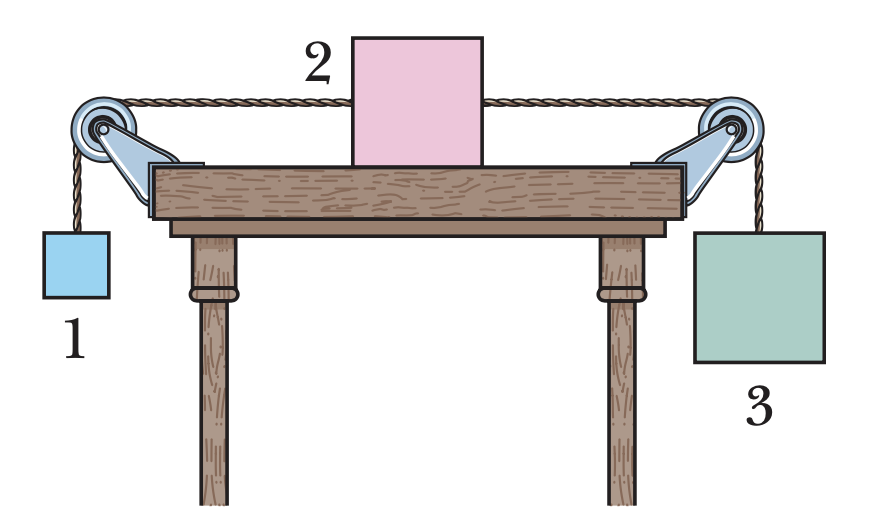
\includegraphics[scale=0.43]{Qfig6-1-20220321.png}  
  \caption{문제 1}
  \label{fig:1}
\end{figure}

\noindent {\bf 풀이}
블록 1과 블록 3에 작용하는 중력의 크기를 각각 $F_1$, $F_2$ 라고 하면,
\begin{align}
  F_1 = Mg,\,\,\, F_2 = 2Mg
\end{align}
이다. 오른쪽을 양의 방향이라 하면 블록 1, 2, 3 에 수평 방향으로 작용하는 힘 $F_{3x}$ 는 
다음과 같다.
\begin{align}
  F_{3x} = 2Mg - Mg - f_k = Mg - f_k
\end{align}
$f_k$ 는 마찰력이다. 블록 2 에 작용하는 수직항력을 $N$ 이라 하면,
\begin{align}
  f_k = \mu_kN.
\end{align}
블록 2에 수직 방향으로 작용하는 힘은 오직 중력 뿐 이므로, 
\begin{align}
  N = 2Mg = 2M\times(9.80\,\mathrm{m/s^2}).
\end{align}
따라서, 블록 1, 2, 3 에 작용하는 합력은 다음과 같다.
\begin{align}
  \begin{split}
    \sum F &= Mg - f_k = Mg - \mu_kN \\
    &= 5M \times (0.500\,\mathrm{m/s^2})
  \end{split}
\end{align}
운동 마찰 계수 $\mu_k$ 는 다음과 같다.
\begin{align}
  \begin{split}
    \mu_k &= \frac{Mg - 5M \times (0.500\,\mathrm{m/s^2})}{N} \\
    &= \frac{M\times((9.80\,\mathrm{m/s^2})-(2.50\,\mathrm{m/s^2}))}
    {2M\times(9.80\,\mathrm{m/s^2})}  \\
    &= 0.372
  \end{split}
\end{align}
운동 마찰 계수는 0.372 이다.
\vspace{2cm}

\noindent {\bf 문제 2 [10pt]} 프라이팬과 달걀 사이의 정지마찰계수는
$\mu_s=0.04$이다. 이 달걀이 프라이팬에서 미끄러지려면 프라이팬은
수평면으로부터 몇 도 기울어져야 하는가?  \\


\noindent {\bf 풀이} 
프라이팬과 수평면이 이루는 각도를 $\theta$ 라고 하자. 달걀에 작용하는 힘을
프라이팬에 수직한 방향과 프라이팬에 평행한 방향으로 분해할 수 있다. 힘의 수직한
방향 성분을 $F_v$, 평행한 방향 성분을 $F_p$ 이라고 하면,
\begin{align}
F_v = mg\cos{\theta},\,\,\,F_p = mg\sin{\theta}  
\end{align} 
이 달걀에 작용하는 수직항력은 $F_v$ 의 반작용이므로 정지 마찰력 $f_s$ 는,
\begin{align}
  \begin{split}
    f_s &= \mu_s N = \mu_s F_v \\
    &= \mu_s mg\cos{\theta}.
  \end{split}
\end{align} 
달걀을 미끄러지게 하는 힘은 $F_p$ 이고 정지 마찰력 $f_s$ 는 이 힘과 반대 방향으로
작용한다. 달걀이 미끄러지기 위해서는 미끄러지게 하는 힘이 정지 마찰력 보다 커야한다. 즉,
\begin{align}
  F_p > f_s
\end{align}
이어야 한다. 따라서,
\begin{align}
  mg\sin{\theta}  > \mu_s mg\cos{\theta}
\end{align}
를 만족하는 가장 작은 $\theta$ 는 다음과 같이 구한다.
\begin{align}
  \frac{1}{\mu_s} = \frac{1}{0.04} > \cot{\theta} .
\end{align}
양변에 $\cot^{-1}$ 을 가해주면,
  \begin{align}
  \theta < \cot^{-1}{\left(\frac{1}{0.04}\right)} \approx 2.30^\circ
\end{align}
이므로 경사각이 $2.30^\circ$ 보다 커지면 달걀이 미끄러진다.
\vspace{2cm}

\noindent {\bf 문제 3 [20pt]}
짐을 실은 승강기의 총 질량이 
$1\,600\,\mathrm{kg}$이다. 초속도 2.00 m/s로 내려오던 승강기가 어느
순간부터 일정한 가속도로 감속하여 5.00 m 더 간 후
정지하였다. 정지하기까지 승강기를 연결한 줄의 장력은 얼마인가? (단,
중력가속도는 $9.80\,\mathrm{m/s^2}$이다.)   
\newpage

{\color{gray} [문제 풀이 쪽]}

\newpage

\noindent {\bf 문제 4 [40pt]} (\textbf{\color{red} 난이도 상})
질량이 각각 $m=16$ kg, $M=88$ kg인 두 블록이 
있다. 그림~\ref{fig:4}처럼 힘 $\vec{F}$를 가해 블록 $m$을 블록 $M$에
맞닿아 있도록 했다. 이 두 블록 사이의 정지마찰계수는
$\mu_s=0.38$이다. 블록 $M$이 놓여있는 수평면과 $M$ 사이에는 쓸림이
없다.  블록 $m$이 블록 $M$에서 미끄러져 내려오지 않도록 하는 데 필요한
최소힘 $\vec{F}$를 구하여라. 
\begin{figure}[ht]
  \centering
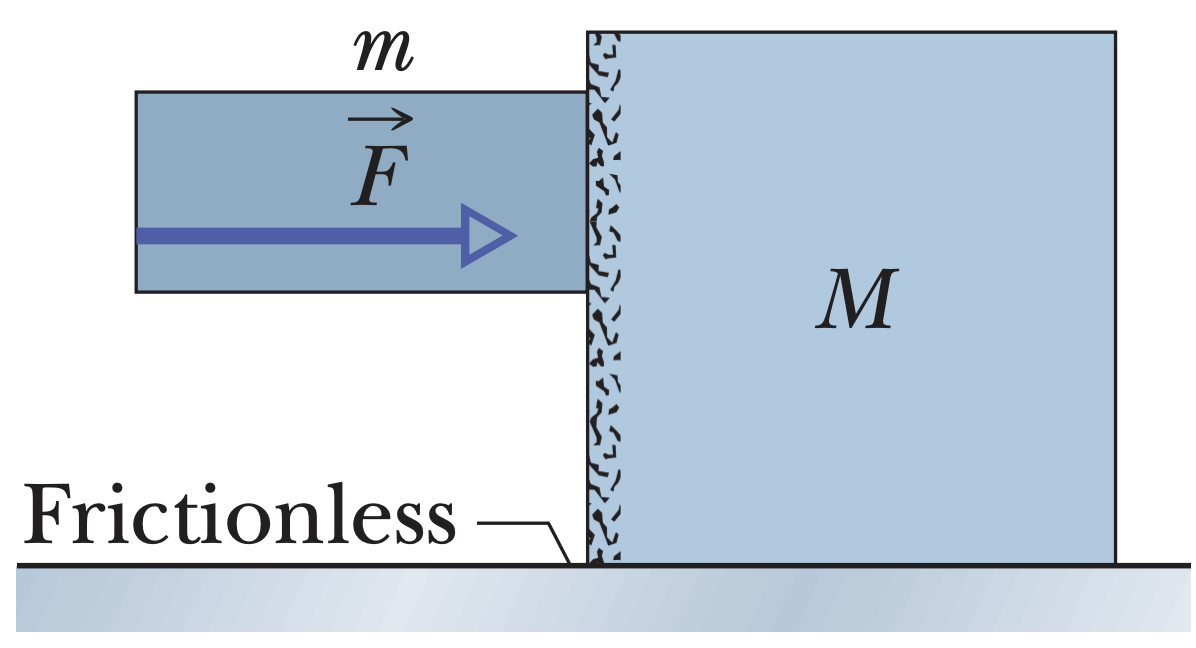
\includegraphics[scale=0.3]{Qfig6-4-20220321.png}  
  \caption{문제 4}
  \label{fig:4}
\end{figure}

\noindent {\bf 풀이} 우선, 블록 $M$ 이 고정되어 움직이지 않을 때 
블록 $m$ 이 떨어지지 않기 위한 최소한의 힘을 $\vec{F_0}$ 라고 하자.
이 때는 수직항력이 $\vec{F_0}$ 이고 물체를 끄는 힘이 중력이므로 블록 $m$ 이
움직이지 않기 위해서는,
\begin{align}\label{eq:4-1}
  \mu_s|\vec{F_0}| = mg,\,\,\, |\vec{F_0}| = \frac{mg}{\mu_s}
\end{align}
이어야 한다. 블록 $M$ 은 움직일 수 있으므로 $\vec{F}$ 가 블록 $M$ 을 움직이도록
하기도 한다. 두 블록은 같이 움직이므로 힘 $\vec{F}$ 가 가해질 때 가속도는,
\begin{align}\label{eq:4-2}
  a = \frac{|\vec{F}|}{M+m}
\end{align}
이다. 블록 $M$ 이 가속하는 원인은 블록 $m$ 이 밀어주는 힘이고 뉴턴의 제 3 법칙에 
의해 블록 $M$ 은 블록 $m$ 에게 같은 크기의 반작용을 가한다. 반작용의 크기를 
$F_{Mm}$ 이라 하면 $F_{Mm}$ 은 정확히 블록 $M$ 이 가속하도록 하는 힘과 같은 크기를
가진다. 따라서,
\begin{align}\label{eq:4-3}
  F_{Mm} = Ma.
\end{align}
블록 $m$ 에 작용하는 합력의 크기는,
\begin{align}
  |\vec{F}|-F_{Mm}
\end{align}
이고, 이 합력이 (\ref{eq:4-1}) 을 만족해야 한다. 즉,
\begin{align}\label{eq:4-4}
  |\vec{F}|-F_{Mm} = \frac{mg}{\mu_s}
\end{align}
이다. $|\vec{F}|$ 를 구해보자. 식 (\ref{eq:4-2}), (\ref{eq:4-3}) 으로 부터,
\begin{align}
  F_{Mm} = Ma = \frac{M|\vec{F}|}{M+m}
\end{align}
이므로,
\begin{align}
  \begin{split}
    |\vec{F}|-F_{Mm} 
    &=|\vec{F}|-\frac{M|\vec{F}|}{M+m}  \\
    &=\left(1-\frac{M}{M+m}\right)|\vec{F}|
  \end{split}
\end{align}
이다. 이를 (\ref{eq:4-4}) 에 대입하면,
\begin{align}
  \left(1-\frac{M}{M+m}\right)|\vec{F}|
  =\left(\frac{m}{M+m}\right)|\vec{F}|
  = \frac{mg}{\mu_s}
\end{align}
이므로,
\begin{align}
  |\vec{F}| = \left(\frac{M+m}{m}\right)\frac{mg}{\mu_s}
  = \frac{(M+m)g}{\mu_s}
\end{align}
이다. $m=16$ kg, $M=88$ kg 과 $\mu_s=0.38$ 를 대입하자.
\begin{align}
  |\vec{F}| = \frac{(88\,\mathrm{kg}+16\,\mathrm{kg})
  (9.8\,\mathrm{m/s^2})}{0.38}
   = 2700\,\mathrm{N}.
\end{align}
블록 $m$ 이 미끄러지지 않기 위해, 최소한 2700 N 의 힘으로 밀어주어야 한다.
\end{document}